\tikzset{
  lb/.style = {font=\tiny},
  nd/.style = {font=\small},
}

\begin{center}
  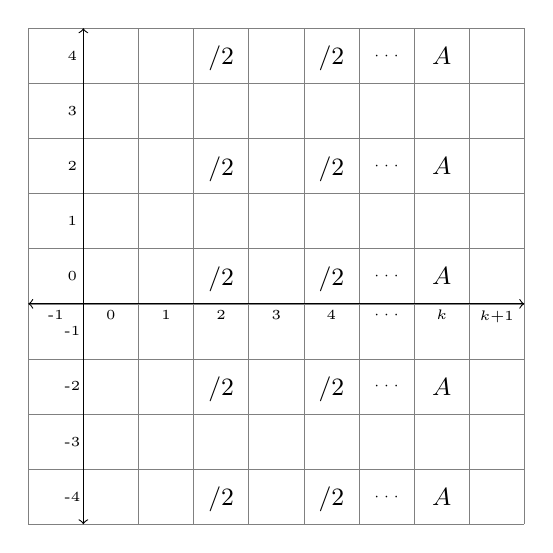
\begin{tikzpicture}[scale=0.7]
    \pgfmathtruncatemacro{\A}{-1}
    \pgfmathtruncatemacro{\B}{7}
    \pgfmathtruncatemacro{\C}{-4}
    \pgfmathtruncatemacro{\D}{4}

    \draw[gray,very thin] (\A,\C) grid (\B+1,\D+1);
    \draw[thin,<->] (0,\C) -- (0,\D+1);
    \draw[thin,<->] (\A,0) -- (\B+1,0);

    \pgfmathtruncatemacro{\E}{\B-3}
    \foreach \x in {\A,...,\E} {
      \node[lb] at (\x+0.5,-0.2) {\x};
    }
    \node[lb] at (\B-1.5,-0.2) {$\cdots$};
    \node[lb] at (\B-0.5,-0.2) {$k$};
    \node[lb] at (\B+0.5,-0.23) {$k$+1};

    \foreach \y in {\C,...,\D} {
      \node[lb] at (-0.2,\y+0.5) {\y};
    }

    \pgfmathtruncatemacro{\F}{\C+2}
    \foreach \y in {\C,\F,...,\D} {
      \node[nd] at (0.5,\y+0.5) {$\Z$};
      \node[lb] at (\B-1.5,\y+0.5) {$\cdots$};
      \node[nd] at (\B-0.5,\y+0.5) {$A$};
      \foreach \x in {2,4,...,\E} {
        \node[nd] at (\x+0.5,\y+0.45) {$\Z/2$};
      }
    }
  \end{tikzpicture}
\end{center}
